\subsection{\Acl{DC}}
The idea of \emph{dual algorithms}, to which \acf{DC} belongs, is similar to \ac{MC}. However, instead of generating polygon vertices on the edges of the cubes, the \ac{DC} method locates them inside the cubes that have vertex values both above and below the isovalues. The basic algorithm can be summarized in these two steps:
\begin{enumerate}
\item Locate the position of the vertex inside each cube.
\item Join the vertices associated with four cubes sharing a common edge, to form a \ac{quad}.
\end{enumerate}
The approach can be seen in \autoref{fig:bunny_MCDC}, with a similar \ac{MC} illustration for comparison.

\begin{figure}
\centering
   \scalebox{0.35}{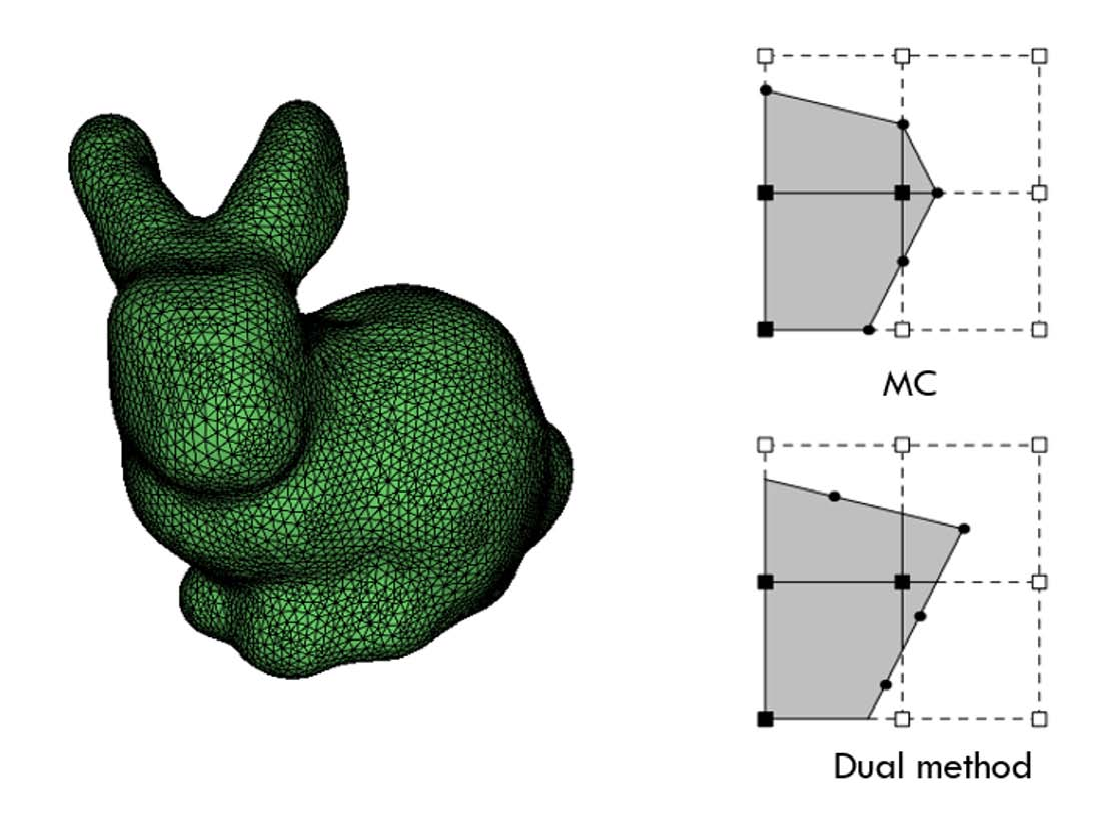
\includegraphics{Pictures/bunny_MC.pdf}}\\
   \caption{\textit{Left:} The famous Stanford Bunny, a popular computer graphics test object, here after application of \ac{MC}. \textit{Right:} Main difference between \ac{MC} and \ac{DC}.  Figures taken from \cite{Hermite2002}. }
   \label{fig:bunny_MCDC}
\end{figure}

\subsubsection{Minimizing the \acl{QEF}}
The relevant question is now where in the cube the ideal place for the vertex is, and here is where different dual algorithms are distinguished. \Ac{DC} in particular generates a vertex positioned at the minimizer of a certain quadratic function, which depends on the (interpolated) isosurface intersection points, as well as the gradient --- or just the normal of the isosurface --- at these points, together the first-order \emph{Hermite data} of the set.
The \acf{QEF}\todo{don't use acronym, but refer to equation number.} for \ac{DC} is defined in \cite{Hermite2002} as follows:
\begin{equation*}
E(x)= x^TA^TAx-2x^TA^Tb+b^Tb
\end{equation*}
where the columns of the matrix \textit{A} are the  isosurface normals at the intersection points, and \textit{b} is a vector containing the scalarproduct of the normals and the intersection points. This system can be solved numerically, for example as proposed in \cite{Hermite2002} by computing the singular value decomposition of \textit{A} and forming the pseudo-inverse, truncating its small singular values. 
The effect of considering the gradient for the calculation of the vertex is huge: \ac{DC} has the ability to represent sharp features like edges and corners, while \ac{MC} often smoothens them away.
\todo[inline]{Benni: explain our approach without hermite data (only root, no gradient, only boolean values) of taking the mean value of the roots, drawbacks of simplification. Do something like a proof why this is resonable.}
In our implementation of \ac{DC} we do not compute the position of the vertex by minimizing the \ac{QEF}, since we cannot access gradient information for our data. Additionally we can only access a discrete dataset with boolean values (determining whether there is material inside the voxel or not) and no function for which we want to compute the isosurface. Therefore we use the following modified approach:
\begin{enumerate}
\item On each voxel edge find the root (i.e. the interface of material and no-material voxels) using bisection.
\item Take the mean value of all root positions for determining the position of the newly introduced vertex.
\end{enumerate}


\subsubsection{Non-manifold surfaces}
One big drawback of \ac{DC} compared to \ac{MC} is that with \ac{DC} we often obtain non-manifold surfaces. A manifold surface is defined by the following topological property:
\begin{quote}
\emph{A $d$-dimensional contour is locally a \emph{manifold} if it is topologically equivalent to a $d$-dimensional disc.}\cite{Hermite2002}
\end{quote}
This means that for 2D data we only get a manifold isocontour, if each vertex is connected to exactly 2 edges\todo{include a figure}. For 3D we only get a manifold isosurface, if each edge is at maximum shared by two \acp{quad}\todo{include a figure}. 

\subsubsection{Topology-safe adaptivity}
Usually having as few faces as possible is desirable for obvious reasons like filesize and complexity of the mesh. But in its basic form \ac{DC} is working with uniformly distributed data and introduces vertices on a uniform grid. The resulting mesh has uniform resolution on the whole area and this results in huge files and a uniformly high resolution, if one wants to resolve fine features of the geometry. As a postprocessing step one could try to simplify the mesh, but especially for \ac{quad} meshes this is a very demanding --- sometimes even impossible --- task\todo{reference}.

The solution to this problem is adaptivity. Referring to \cite{Hermite2002} it is possible to implement \ac{DC} in an adaptive and even topology-safe way. This means we can simplify a \ac{DC} mesh and therefore reduce the number of \acp{quad} needed to represent the surface, while still conserving the topological structure of our surface.